\pagestyle{plain}  % kvuli cislovani stranek

\chapter{Nástroje pro modelování multi-modelových dat}

V následující kapitole rozebereme problémy multi-modelových dat, podíváme se detailněji na MM-cat framework a stručně rozebereme jeho grafické rozhraní.

Nové typy databázových systémů, jako jsou NoSQL databáze, přinášejí další logické modely pro ukládání dat. Tyto systémy umožňují vytvářet databáze na základě modelů, jako jsou: klíč-hodnota, dokumentové nebo grafové.

Zatím neexistuje dostatečná standardizace pro propojení modelů. O řešení se snaží multi-modelové databáze. Do jednoho systému lze začlenit více modelů tak, že spolu koexistují v různých vzájemně propojených formátech a modelech. Propojení může fungovat různými způsoby. Jeden model může být vložen do druhého, entity z jednoho můžou ukazovat na entity z druhého, nebo redundance dat může být uložena ve více modelech. Stále ale neexistuje obecný způsob, jak modelovat multi-modelová data, nebo je transformovat z jednoho modelu do druhého.

Existuje přístup, který využívá teorii kategorií (category theory) k formálnímu zachycení reprezentace a transformace multi-modelových dat \cite{cat_theory}. Tento přístup umožňuje propojení různých modelů a volbu jejich kombinace. Další výhodou je jednotné dotazování nad daty, migrace mezi modely a evoluce modelu i dat. Vše by mělo být možné bez znalosti specifik propojených modelů. Tímto přístupem je teké docíleno určité jednoduchosti v návrhu, protože teorii kategorií lze převést na grafovou reprezentaci, což by mělo usnadnit praktické využití.

Na základě přístupu, který využívá teorii kategorií, bylo vyvinuto několik návrhů funkcionalit a nástrojů, které na něm staví. Například nástroj MM-infer se snaží schéma zpětně zrekonstruovat z~již uložených multi-modelových dat \cite{MM_infer}. Taková funkčnost se nám může hodit, když data nemají předem definované schéma. Nástroj MM-quecat ukazuje, jak se dotazovat nad multi-modelovými daty \cite{MM_quecat} a MM-evocat navrhuje evoluci dat \cite{MM_evocat}. Vše by mělo být nezávislé na propojených databázových systémech. Nás bude ale hlavně zajímat nástroj MM-cat, jehož specifika rozebereme v následující sekci.

\section{MM-cat}

MM-cat framework je navržený tak, aby řešil složitosti spojené s~návrhem a~správou multi-modelových databází. Jeho hlavním úkolem je vytvářet kategorický model (multi-modelové schéma). Umí ho dekomponovat a~umožňuje uživateli, aby si zvolil mapování na příšlušné DBMS (Database Management System).

Postupně byla do MM-cat frameworku zaintegrována i funkčnost MM-evocat. Díky tomu umí řešit případy, kdy se struktura dat v~čase mění tak, aby například vyhovovala novým uživatelským požadavkům. Takové změny jsou pak propagovány napříč definovanými modely a~datovými instancemi. Dál se do frameworku postupně přidává i odvozování schématu a dotazování nad multi-modelovými daty.

MM-cat je framework, který má zatím nedokončené grafické webové rozhraní. Při vzniku nástroje nebyl kladený důraz na jeho návrh a možnosti dalšího rozšíření. Proto se následující práce zabývá návrhem nového uživatelského rozhraní, které má být vytvořeno nezávisle na existujícím.

\subsection{Stručná analýza grafického rozhraní}

Cílem této sekce není provádět podrobnou analýzu stávajícího rozhraní. Snažíme se vypíchnout hlavní nedostatky současného návrhu, které jsou jedním z důvodů pro vytvoření nového nezávislého rozhraní.

Jedním z prvních technických nedostatků je, že design webu není responzivní. Občas se stává, že na různých velikostech obrazovky nejsou části nástroje správně zobrazeny nebo jsou zakryté. Je to určitě jedna z věcí na kterou implementaci nového návrhu budeme dbát.

Dále pro nástroj chybí sjednocená grafická knihovna. Postupným přidáváním dalších funkcionalit se navíc různě používalo stylování. Některé části jsou vytvořené pomocí vlastního CSS, jiné využívají Bootstrap framework.

Pro lepší pochopení a vizualizaci si rozebereme ukázku ze současného rozhraní MM-cat. Podíváme se na otevřené schéma (Obr. \ref{obr01:mm-cat}) ve webové aplikaci. V pravé i levé dolní liště se objevují tlačítka, která často nemají žádnou funkci. Jak fungují je potřeba najít v dokumentaci. Levá lišta se mění na jinou po přístupu do jiných částí aplikace, což alespoň ze začátku používání aplikace může být matoucí.

\begin{figure}[htb]
  \centering
  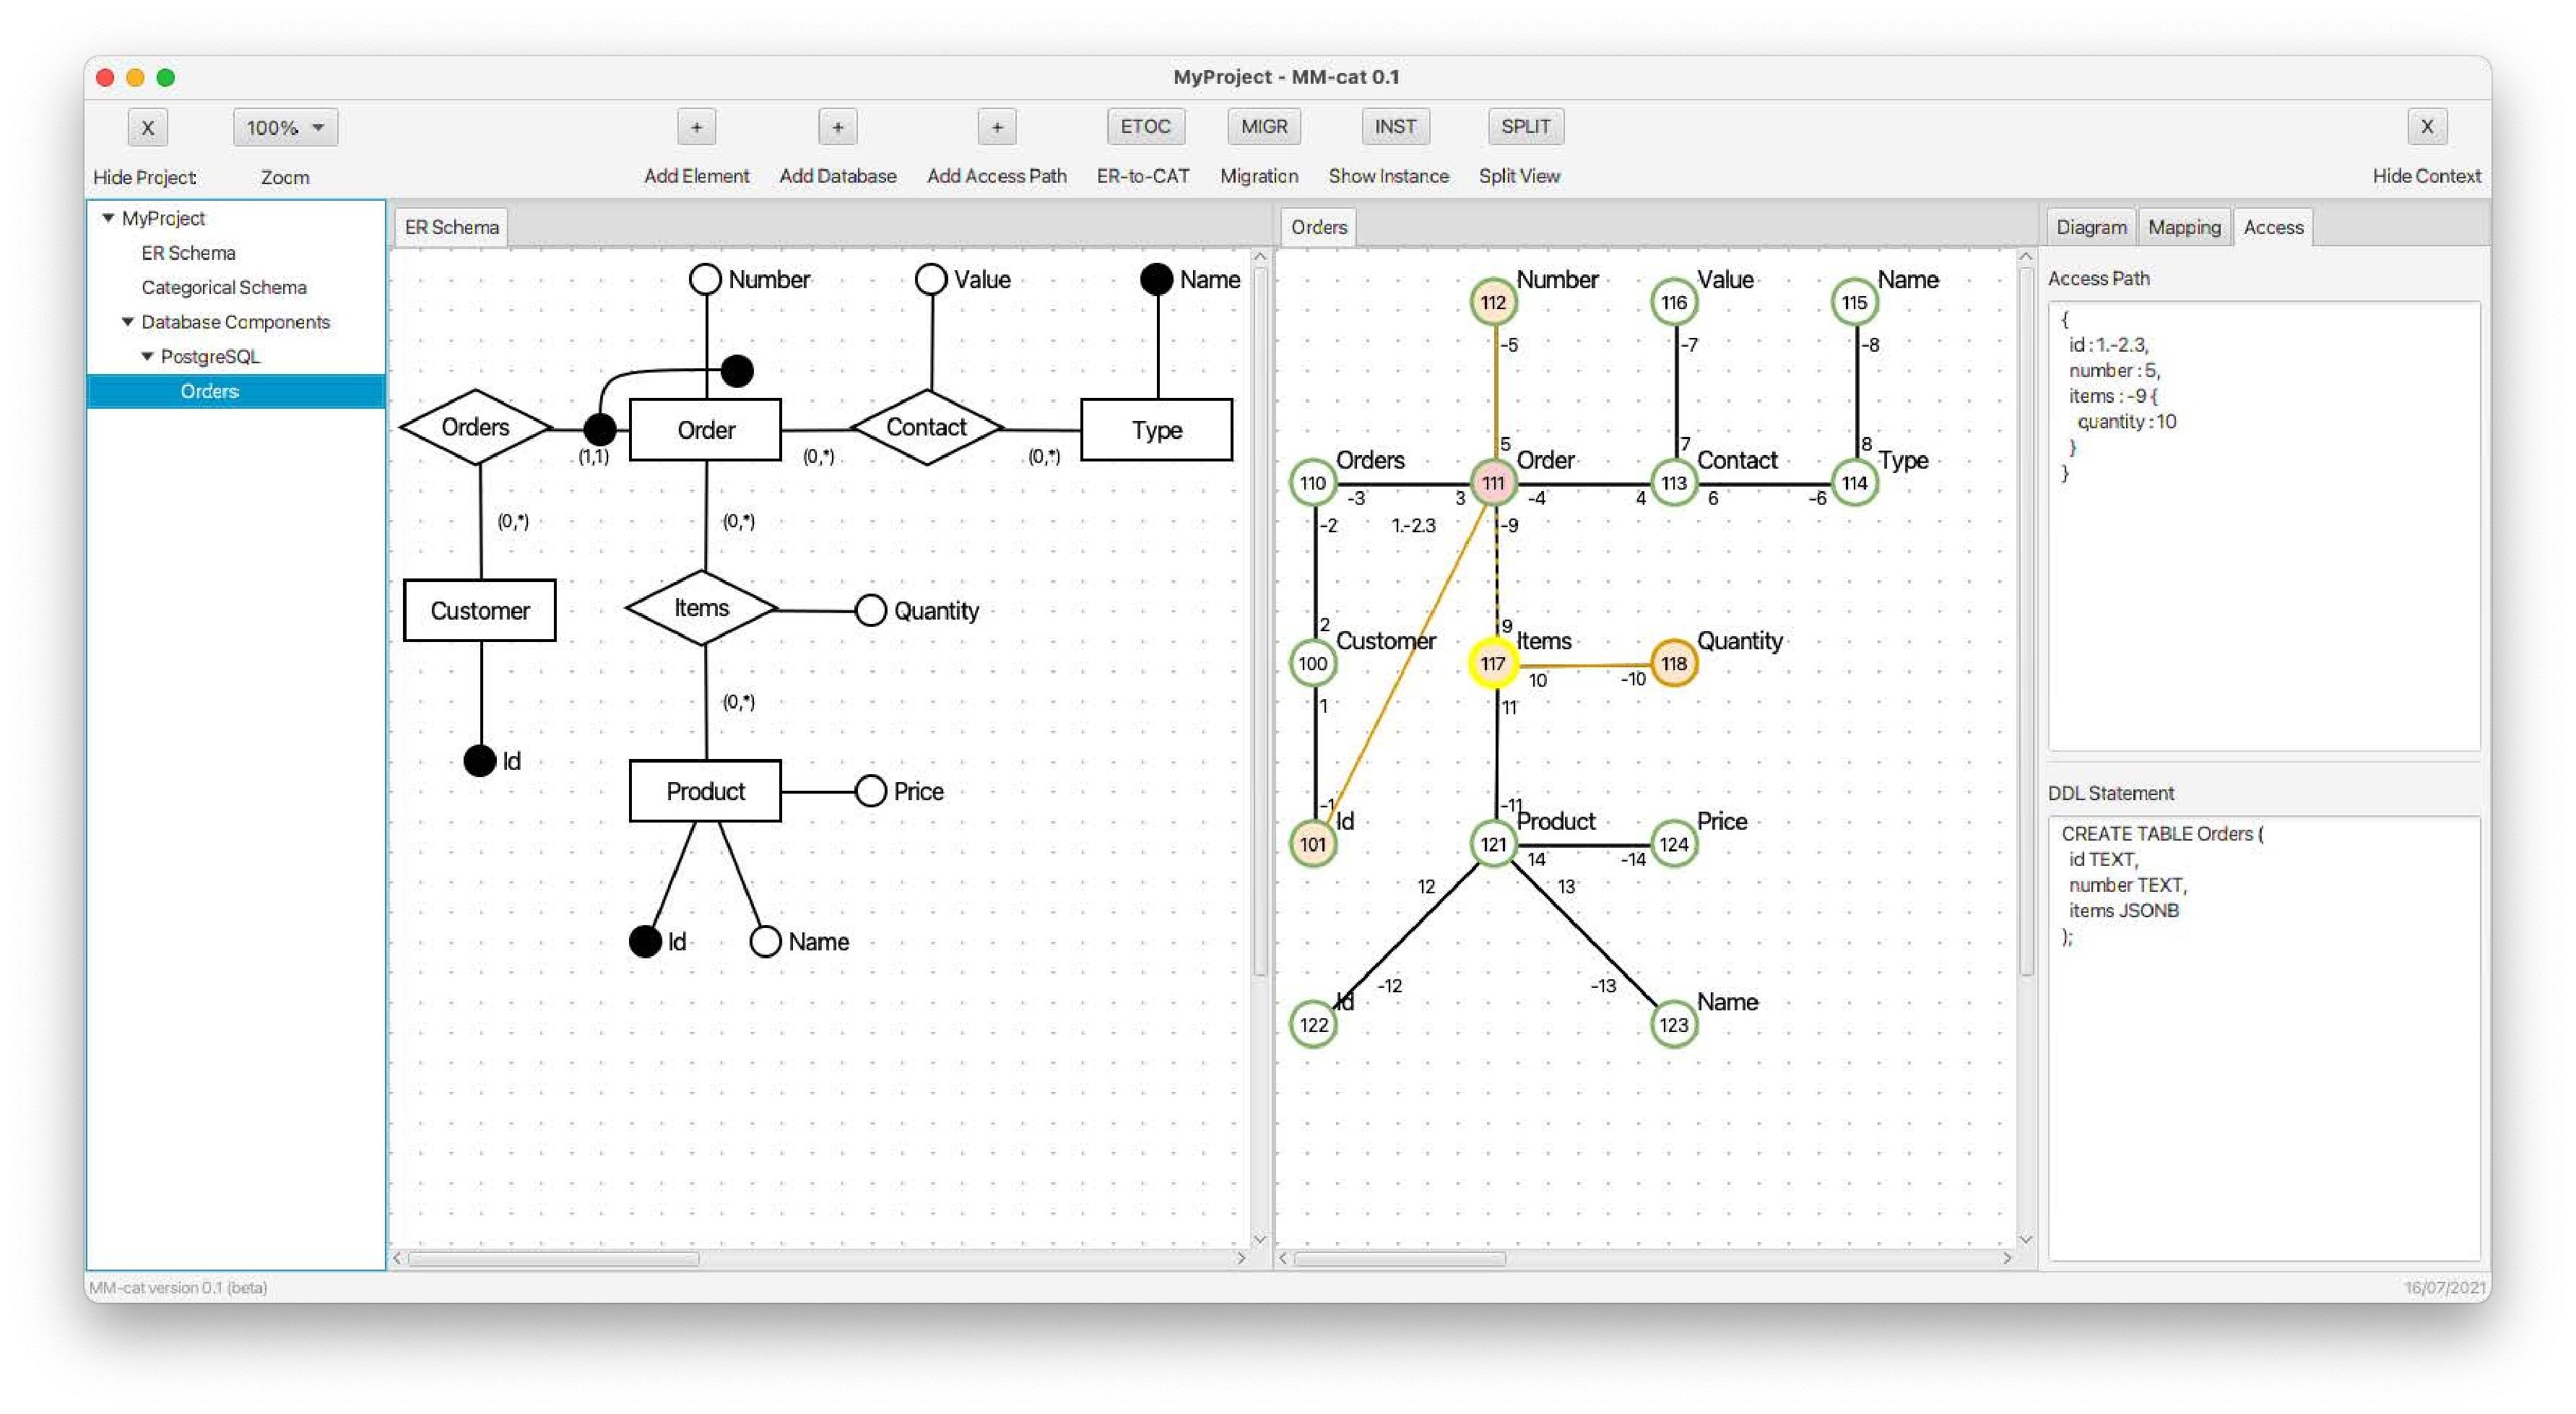
\includegraphics[height=90mm]{../img/mm-cat}
  \caption{Ukázka uživatelského rozhraní nástroje MM-cat.}
  \label{obr01:mm-cat}
\end{figure}

V horní liště je pak umístěný název otevřeného schématu „Basic Schema“. Pozice v liště, která vypadá jako navigační menu, nemusí být intuitivní. Na další omezení a nejasnosti uživatel narazí při dalším používání. Často je potřeba podívat se do dokumentace, co vlastně nástroj dělá a umí.

Pro všechny vyjmenované důvody, a také s cílem zjednodušit integraci dalších nástrojů, se snažíme navrhnout nové sjednocené grafické rozhraní.
